\chapter{Cloud Archive}

The Gravwell Cloud Archive Service allows old data to be moved from
active indexers to a separate archive service. Once archived, data can
still be accessed by creating a temporary Gravwell instance in Docker.

The reference implementation accepts uploaded shards from indexers and
archives them to the filesystem. This is designed to be somewhat
modular, allowing implementation of different storage and authentication
strategies if desired.

\section{Architectural Overview}

A cloud archive system consists of two components: the archive server
and some set of indexers. The archive server receives archived shards
from the indexers. Indexers send aged-out shards to the archive server,
then delete them locally; after a shard has been uploaded to the archive
server, all responsibility for the storage and management of that shard
is transferred from the indexer to the archive server.

\subsection{Archive Server}

The archive server is a standalone process which listens for incoming
HTTPS connections from Gravwell indexers. It performs the following
functions:

\begin{itemize}
\item
  Authenticates indexers as they connect
\item
  Archives shards sent by the indexers
\end{itemize}

The server is configured via a file (specified with the \code{-config-file}
option when launching the server) which looks like this:

\begin{Verbatim}[breaklines=true]
[Global]
Listen-Address="0.0.0.0:443"
Cert-File=/path/to/cert.pem
Key-File=/path/to/key.pem
Password-File=/path/to/cloud.passwd
Log-Level=INFO
Storage-Directory=/path/to/archive/
\end{Verbatim}

The Listen-Address field specifies upon which IP and port to listen for
incoming connections. The Cert-File and Key-File parameters should point
to a valid X509 certificate/key pair. The Password-File field
points to a file which contains authentication information for clients;
see below for more info on authentication. The Log-Level parameter
specifies how verbosely it should log, and the optional Log-File
parameter allows logging to be sent to a file rather than the terminal.
Finally, the Storage-Directory parameter is used to configure where
shards are stored.

\subsection{Indexers}

Gravwell indexers must be configured before they can send shards to the
archive server. Configuration consists of a system-wide specification
which gives the archive server's address and authentication information,
plus a per-well configuration option which enables archiving on that
well. The system-wide specification looks like this:

\begin{Verbatim}[breaklines=true]
[Cloud-Archive]
Archive-Server="archive.example.org:443"
Archive-Shared-Secret="ArchiveSharedSecret"
\end{Verbatim}

Setting the system-wide configuration allows the indexer to talk to the
archive server, but nothing will be \emph{archived} unless the
\code{Archive-Deleted-Shards} option is set to true on a well. With that
option set, whenever the indexer decides to delete a shard within that
well (as controlled by the \code{Delete-Cold-Data} and
\code{Delete-Frozen-Data} config options), it will first send the shard to
the archive server.

\section{Reference Service Implementation}

Although source code is provided to implement custom archive servers,
Gravwell provides a reference implementation which should be suitable
for basic use. The reference archive server stores archived shards on
the local filesystem and authenticates incoming indexers using an
on-disk password file.

\subsection{Filesystem Storage}

The example instance stores archived shards on the local filesystem.
Under the directory specified by the Storage-Directory parameter of the
configuration file, the server establishes a hierarchy of directories
with the structure \code{\textless{}customer
id\textgreater{}/\textless{}indexer uuid\textgreater{}/\textless{}well
name\textgreater{}/\textless{}shard id\textgreater{}}. For example, if
the customer with customer number 1234 configures an indexer with
the UUID 39c1ba74-851c-4951-b409-a1909fba37e8 to archive its default
well, the directory
\code{1234/39c1ba74-851c-4951-b409-a1909fba37e8/default/} will contain
shards from that indexer's default well.

This structure makes it trivial to instantiate a new Gravwell instance
using archived data from any given indexer, since the directory
structure under each individual indexer's directory mirrors Gravwell's
live storage structure. See below for a demonstration.

\subsection{File-based Authentication}

Authentication is handled via a passwd-style file specified with the
\code{Password-File} directive in the webserver configuration. The password
file contains an encrypted password for each customer to use when
authenticating to the webserver. It can be managed with the usertool
utility:

\begin{Verbatim}[breaklines=true]
$ ./usertool -h
Usage of ./usertool:
  -action string
        action to take (list, useradd, userdel, passwd) (default "list")
  -id uint
        User ID
  -passfile string
        Path to the password file
  -password string
        Password to use when adding a user, if blank you will be prompted
\end{Verbatim}

Thus, to add a new user with the customer id 1234, one might specify:

\begin{Verbatim}[breaklines=true]
usertool -action useradd -passfile /path/to/cloud.passwd -id 1234 -password Customer1234ArchiveSecret
\end{Verbatim}


\section{Binding to Archived Shards}

The Gravwell Cloud Archive service is designed to store uploaded shards
in a format that allows another instance of Gravwell to use them
directly. The reference implementation stores the uploaded shards to a
directory on the local filesystem. An example use case might be a
commercial service where customers deploy local Gravwell instances on
premises and an OEM provider hosts a remote archive system. The stored
shards are fully dormant, but should a customer decide that they need to
query data in the old shards, they can request that the OEM provider
dynamically instantiate a Gravwell instance and bind it to their stored
data. 

This section will demonstrate using some basic Docker commands and the
configuration package to start a Gravwell instance which can directly
operate on those shards. Using the demonstration implementation
provided we will dynamically generate a configuration file which matches
the archived data and start a Gravwell instance as a Docker container.
The container will allow the remote customer to execute queries against
their old data on the remote system. When the customer is done
executing queries, the Gravwell instance can be terminated. The stored
data remains and CPU and memory resources are only allocated when
customers explicitly need them.

\subsection{Reference Implementation Directory Structure}

Our example directory listing shows the directory structure for a
sample customer with customer ID 1234 and two active indexers. This
customer is archiving the default well and two custom wells from each
indexer; each well has archived out three shards of old data.

\begin{Verbatim}[breaklines=true]
1234                  
   |-007d25c3-ad5d-4b50-b870-80d6c812a33f
   |---tags.dat
   |---default
   |-----76a06
   |-----76a07
   |-----76a08
   |-----tags
   |---cef            
   |-----76a06
   |-----76a07        
   |-----76a08
   |-----tags                           
   |-1fcd3c24-36c4-493b-a16a-1deaa7ac8c78
   |---tags.dat
   |---default
   |-----76a07
   |-----76a08
   |-----tags
\end{Verbatim}

\subsection{Configuration Generation}

The reference Cloud Archive system contains a Go package named
\code{configbuilder} and a simple tool named \code{configtool} which
demonstrates its use. The \code{configbuilder} package is used to
dynamically generate a gravwell.conf based on the archived data.
For the purpose of this example we will use the
configtool application, but a well-integrated system would use the
configbuilder package directly.

The configbuilder package expects a `stub' file which contains some
basic gravwell.conf parameters. The package then adds well configurations
to this stub. To generate a gravwell.conf file for customer
1234 and indexer 007d25c3-ad5d-4b50-b870-80d6c812a33f we provide
the configtool the stub file and the full path to the base of the
indexer. For this example the full path is
\code{/mnt/gravwell/1234/007d25c3-ad5d-4b50-b870-80d6c812a33f}.

\begin{Verbatim}[breaklines=true]
./configtool -o /dev/shm/gravwell.conf -stub stub \
-dir /mnt/gravwell/1234/19cf4a65-6505-4da9-ae77-a0d0ef50d1a3
\end{Verbatim}

The stub file configuration file contains a minimal set of
configuration variables that can be adjusted as needed. Of particular
note is the \code{Tag-DB-Path} parameter which changes the default location
of the \code{tags.dat} file. Each Gravwell indexer must have a consistent
tag mapping file in order to correctly map a tag name to the internal
tag ID. The cloud archive system ships an updated tag mapping with each
Cloud Archive update, which is stored at the base of the indexer
directory structure. Each shard update also contains the current set of
tags that are assigned to that well, which allows the
configbuilder package to appropriately assign tags to wells.

Our example stub file is:

\begin{Verbatim}[breaklines=true]
[global]
Indexer-UUID=00000000-0000-0000-0000-000000000000
Ingest-Auth=IngestSecrets
Control-Auth=ControlSecrets
Search-Agent-Auth=SearchAgentSecrets
Web-Port=80
Insecure-Disable-HTTPS=true
Remote-Indexers=net:127.0.0.1:9404
Persist-Web-Logins=True
Session-Timeout-Minutes=1440
Search-Pipeline-Buffer-Size=4
Log-Level=INFO
Tag-DB-Path=/opt/gravwell/storage/tags.dat
\end{Verbatim}


After invoking the configtool the output \code{gravwell.conf} file is:

\begin{Verbatim}[breaklines=true]
[global]
Indexer-UUID=19cf4a65-6505-4da9-ae77-a0d0ef50d1a3
Ingest-Auth=IngestSecrets
Control-Auth=ControlSecrets
Search-Agent-Auth=SearchAgentSecrets
Web-Port=80
Insecure-Disable-HTTPS=true
Remote-Indexers=net:127.0.0.1:9404
Persist-Web-Logins=True
Session-Timeout-Minutes=1440
Search-Pipeline-Buffer-Size=4
Log-Level=INFO
Tag-DB-Path=/opt/gravwell/storage/tags.dat

[Default-Well]
        Location=/opt/gravwell/storage/default
[Storage-Well "cef"]
        Location=/opt/gravwell/storage/cef
        Tags=cef
        Tags=cef1
        Tags=cef2
        Tags=cef3
[Storage-Well "syslog"]
        Location=/opt/gravwell/storage/syslog
        Tags=syslog
        Tags=syslog1
        Tags=syslog2
        Tags=syslog3
\end{Verbatim}

\subsection{Configuring Docker Instance}

We now have a directory structure containing many customers and
indexers. We also have a method to generate an appropriate configuration
file given a customer and indexer directory. For this section we will
demonstrate a few Docker commands to dynamically create a running
Gravwell Docker instance and bind it to the cloud archive data. The
Docker instance will be able to search the archived data as if it was
its own. We will demonstrate binding a single Gravwell instance
(non-cluster) to archive data; the process for standing up a cluster
instance with multiple indexers and a single webserver may require that
some configuration parameters be passed in on the fly using Docker
secrets. See https://docs.gravwell.io/\#!configuration/docker.md
for additional information on passing configuration information at
runtime.

Other platforms based on Docker containers (such as Kubernetes or
Redhat OpenShift) can achieve similar results. We will be using Docker
commands directly, but interacting via the Docker API (or Kubernetes, or
Openshift APIs) would for better control and error handling.

\subsubsection{Creating The Container}

The first step is to create a new container. We will be targeting
customer 1234 and indexer 19cf4a65-6505-4da9-ae77-a0d0ef50d1a3.

\begin{Verbatim}[breaklines=true]
docker create --name 1234_archive_access \
-v /mnt/gravwell/1234/19cf4a65-6505-4da9-ae77-a0d0ef50d1a3\
:/opt/gravwell/storage gravwell/gravwell:latest
\end{Verbatim}

The command creates a new container with
\code{/opt/gravwell/storage} directly mapped to the Cloud Archive storage
location for the specified customer and indexer. The container is not
yet running, so we can copy in the gravwell.conf file we generated
earlier, as well as a valid license.

\begin{Verbatim}[breaklines=true]
docker cp /path/to/123/cloud/license 1234_archive_access:/opt/gravwell/etc/
docker cp /path/to/gravwell.conf 1234_archive_access:/opt/gravwell/etc/
\end{Verbatim}


Our container is now ready to start.

\begin{Verbatim}[breaklines=true]
docker start 1234_archive_access
\end{Verbatim}

If all has gone well, the Gravwell instance will be running with access
to all cloud archive data.

\textbf{WARNING}: The gravwell instance is in a default state with a default
admin password ``changeme''. Additional steps should be taken to
change the admin password or limit access to the instance. Directly
exposing the newly started container to the public Internet will expose
your customer's data.

\section{Hands-on Lab: Cloud Archive}

This lab will stand up a Gravwell indexer and a Gravwell Cloud Archive
server, then show how the indexer can archive old shards to the cloud
archive server.

We'll use a working directory in our training directory for these
operations, allowing easy cleanup:

\begin{Verbatim}[breaklines=true]
cd ~/gravwell_training/CloudArchive/
\end{Verbatim}

\subsection{Archiving Shards}

First, launch a Gravwell webserver+indexer container:

\begin{Verbatim}[breaklines=true]
docker run --rm --net gravnet -p 8080:80 -d --name gravwell gravwell:base
\end{Verbatim}

Next, we'll use the ingesters container to feed some entries into the
indexer using the JSON generator. We'll specify that the entries should
cover 10 days:

\begin{Verbatim}[breaklines=true]
docker run --net gravnet --rm -it --name ingesters \
gravwell:ingesters /opt/gravwell/bin/jsonGenerator \
-clear-conns gravwell:4023 -entry-count 100000 -duration 10d
\end{Verbatim}

We can verify that there are several shards in the default well at this
point:

\begin{Verbatim}[breaklines=true]
$ docker exec -it gravwell ls -l /opt/gravwell/storage/default
total 28
drwxr-xr-x    2 root     root          4096 Mar 19 19:20 76a0b
drwxr-xr-x    2 root     root          4096 Mar 19 19:20 76a0c
drwxr-xr-x    2 root     root          4096 Mar 19 19:19 76a0d
drwxr-xr-x    2 root     root          4096 Mar 19 19:19 76a0e
drwxr-xr-x    2 root     root          4096 Mar 19 19:19 76a0f
drwxr-xr-x    2 root     root          4096 Mar 19 19:19 76a10
drwxr-xr-x    2 root     root          4096 Mar 19 18:05 76a11
\end{Verbatim}

Now we'll stand up a cloud archive server:

\begin{Verbatim}[breaklines=true]
docker run --rm --net gravnet -d \
--name cloudarchive gravwell:cloudarchive
\end{Verbatim}

In order for the indexer to authenticate with the cloud archive server,
the archive server must have an entry added to its password database.
First, look up your customer number by selecting the ``License'' page on
the Gravwell GUI, as shown in Figure \ref{fig:cust-num}.

\begin{figure}
	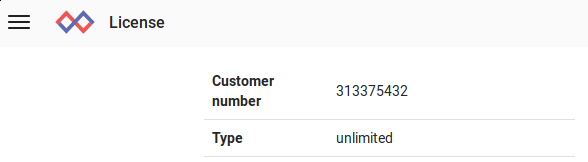
\includegraphics{images/cust-num.png}
	\caption{Customer number}
	\label{fig:cust-num}
\end{figure}

Then run the following command to add an entry for your customer number
on the cloud archive server, replacing YOUR\_CUSTOMER\_NUMBER with the
number you found on the License page:

\begin{Verbatim}[breaklines=true]
docker exec -it cloudarchive /opt/gravwell/bin/usertool \
-passfile /opt/gravwell/etc/cloud.passwd -action useradd \
-id YOUR_CUSTOMER_NUMBER -password CloudArchiveSecrets
\end{Verbatim}

The archive server is listening on port 8886, so edit gravwell.conf on
the webserver+indexer container and add the following just above the
\code{[Default-Well]} section:

\begin{Verbatim}[breaklines=true]
[Cloud-Archive]
Archive-Server="cloudarchive:8886"
Archive-Shared-Secret="CloudArchiveSecrets"
Insecure-Skip-TLS-Verify=true
\end{Verbatim}

Then modify the \code{[Default-Well]} section to look like this:

\begin{Verbatim}[breaklines=true]
[Default-Well]
        Location=/opt/gravwell/storage/default/
        Archive-Deleted-Shards=true
        Hot-Duration=2d
        Delete-Cold-Data=true
\end{Verbatim}

And restart the indexer:

\begin{Verbatim}[breaklines=true]
docker exec -it gravwell killall gravwell_indexer
\end{Verbatim}

Normally, indexers only age-out shards after running for at least 10
minutes. We will accelerate this process by sending the SIGUSR2 signal:

\begin{Verbatim}[breaklines=true]
docker exec -it gravwell killall -s SIGUSR2 gravwell_indexer
\end{Verbatim}

You should quickly see the shards migrated off the indexer:

\begin{Verbatim}[breaklines=true]
$ docker exec -it gravwell ls -l /opt/gravwell/storage/default
total 8
drwxr-xr-x    2 root     root          4096 Mar 19 21:12 76a10
drwxr-xr-x    2 root     root          4096 Mar 19 21:12 76a11
\end{Verbatim}

And onto the cloud archive:

\begin{Verbatim}[breaklines=true]
$ docker exec -it cloudarchive du -hs /opt/gravwell/cloud_archive
95.8M    /opt/gravwell/cloud_archive
\end{Verbatim}

\subsection{Binding to Archived Shards}

The archived shards can be re-instantiated into another Gravwell
container at a later date. In this portion of the lab, we will show how
to generate a gravwell.conf for the shards we just archived and stand up
a new Gravwell container to access them.

Copy the cloud archive stub file into the cloudarchive container:

\begin{Verbatim}[breaklines=true]
cd ~/gravwell_training/CloudArchive/Lab-Archive/
docker cp config/cloudarchive-stub.conf cloudarchive:/tmp/
\end{Verbatim}

Then get a shell on the cloudarchive container and find the UUID of
the indexer which archived the shards. This will differ every time!

\begin{Verbatim}[breaklines=true]
$ docker exec -it cloudarchive /bin/sh
/ # cd /opt/gravwell/cloud_archive/
/opt/gravwell/cloud_archive # ls
313375432
/opt/gravwell/cloud_archive # ls 313375432/
178f94bc-eb91-4f12-ad55-f09f18bd63b2
\end{Verbatim}

The example above shows that customer number 313375432 archived
shards from the indexer with the UUID
178f94bc-eb91-4f12-ad55-f09f18bd63b2. Substitute your own values
into the command below and run it:

\begin{Verbatim}[breaklines=true]
docker exec -it cloudarchive /opt/gravwell/bin/configtool \
-o /tmp/archive-gravwell.conf -stub /tmp/cloudarchive-stub.conf \
-dir /opt/gravwell/cloud_archive/313375432/178f94bc-eb91-4f12-ad55-f09f18bd63b2
\end{Verbatim}

This will generate a Gravwell configuration in
\code{/tmp/archive-gravwell.conf} on the cloudarchive container. Now we'll
create a new Gravwell instance and copy in the data from the
cloudarchive container. Be sure to substitute your own customer
number and UUID into the commands below!

\begin{Verbatim}[breaklines=true]
docker run --rm --net gravnet -p 8081:80 --name gravarchive gravwell:base

docker cp cloudarchive:/tmp/archive-gravwell.conf .
docker cp archive-gravwell.conf gravarchive:/opt/gravwell/etc/gravwell.conf

docker cp \
cloudarchive:/opt/gravwell/cloud_archive/\
313375432/178f94bc-eb91-4f12-ad55-f09f18bd63b2/tags.dat .
docker cp tags.dat gravarchive:/opt/gravwell/etc/

docker cp \ 
cloudarchive:/opt/gravwell/cloud_archive/\
313375432/178f94bc-eb91-4f12-ad55-f09f18bd63b2/default .

docker exec cloudarchive mkdir -p \
/opt/gravwell/cloud_archive/313375432/178f94bc-eb91-4f12-ad55-f09f18bd63b2/

docker cp default \
gravarchive:/opt/gravwell/cloud_archive/313375432/178f94bc-eb91-4f12-ad55-f09f1\
8bd63b2/

docker restart gravarchive
\end{Verbatim}

Now point your browser to
\href{http://localhost:8081/}{http://localhost:8081/}, log in and run the query
\code{tag=json} over the last week. You should see entries starting from
approximately two days before.

To clean up after the experiment, simply run:

\code{docker kill \$(docker ps -a -q)}
